 
%
% $Id: slides.tex 4228 2006-06-21 21:55:12 rocapal $
%
%
% Compilar a .pdf con LaTeX (pdflatex)
% Es necesario instalar Beamer (paquete latex-beamer en Debian)
%



\documentclass{beamer}
\usetheme{Warsaw}
\usebackgroundtemplate{
\includegraphics[width=\paperwidth]{format/libresoft-bg.png}}
\usepackage[english]{babel}
\usepackage[latin1]{inputenc}
\usepackage{graphics}
\usepackage{amssymb} % Simbolos matematicos
\usepackage{url}
%\usepackage{html}
%\usepackage{hthtml}

%\definecolor{libresoftgreen}{RGB}{162,190,43}
%\definecolor{libresoftblue}{RGB}{0,98,143}

%\setbeamercolor{titlelike}{bg=libresoftgreen}

%% Metadatos del PDF.
\hypersetup{
  pdftitle={Android Platform},
  pdfauthor={Roberto Calvo Palomino},
  pdfcreator={GSyC/Libresoft},
  pdfproducer=PDFLaTeX,
  pdfsubject={nn},
}
%%


\AtBeginSection[]
{
  \begin{frame}<presentation>
    \frametitle{Index}
    \tableofcontents[current]
  \end{frame}
}


\begin{document}

\title{Android: Project \& Community }
%\subtitle{Curso de Desarrollo en Android}
\subtitle{Modulo 5: Android}
\institute{\\rocapal@libresoft.es\\
GSyC/Libresoft}
\author{Roberto Calvo}
\date{\today}

\frame{
\maketitle
\begin{center}

\includegraphics[width=6cm]{format/gsyc-urjc}
\hspace{0.5cm}

\includegraphics[width=2.5cm]{format/eoi}
\end{center}
}


%\title{Titulo corto}
%\author{Autores abreviado}


%% LICENCIA DE REDISTRIBUCION DE LAS TRANSPAS
\frame{
~
\vspace{4cm}

\begin{flushright}
{\tiny
(cc) 2011 Roberto Calvo Palomino. \\
Some rights reserved. This document is distributed under the Creative \\
            Commons Attribution-ShareAlike 2.5 licence, available in \\
            http://creativecommons.org/licenses/by-sa/2.5/

}
\end{flushright}
}


\section{Introduction}

\begin{frame}
\frametitle{Terms}
\begin{itemize}
\item Google: Company extremely well-known
\item Android: is an operative system
\item HTC: is a mobile hardware company
\item T-Mobile: is a mobile network operator (Germany) 
\item HTC Dream / G1: First android mobile phone
\item HTC Magic / G2: Second android mobile phone
\item Nexus S and Galaxy Nexus: The bests android mobile phones
\end{itemize}
\end{frame}

\begin{frame}
\frametitle{Open Handset Alliance}
\begin{itemize}
\item The Open Handset Alliance (OHA) is a business alliance of 47
  firms including Google, HTC, Intel, Motorola, Qualcomm, Samsung, LG,
  T-Mobile, Nvidia and Wind River Systems to develop open standards
  for mobile devices.
\item Members: Mobile operators, Software companies, Commercialization
  companies, Semiconductor companies and Handset companies.

\begin{center}
\htmladdnormallink{OHA in wikipedia}{http://en.wikipedia.org/wiki/Open_Handset_Alliance}
\end{center}
\end{itemize}
\end{frame}


\section{Android}


\begin{frame}
\frametitle{Introduction}

Android is a software stack for mobile devices that includes an
operating system, middleware and key applications. The Android SDK
provides the tools and APIs necessary to begin developing applications
on the Android platform using the Java programming language.

\end{frame}

\begin{frame}
\frametitle{Features}
\begin{itemize}
\item Apache License 2.0
\item Android relies on Linux version 2.6
\item Dalvik virtual machine optimized for mobile devices 
\item Optimized graphics (2D graphics library); 3D
  graphics based on the OpenGL
\item SQLite for structured data storage
\item Bluetooth, 3G, and WiFi, NFC (hardware dependent)
\item Camera, GPS, compass, and accelerometer (hardware dependent)
\item Device emulator, tools for debugging, and a plugin for the Eclipse IDE
\end{itemize}
\end{frame}

%\begin{frame}
%\frametitle{License}
%Apache 2.0 License:
%\begin{itemize}
%\item permissive or copyleft license ??
%\item Business models.
%\end{itemize}
%\end{frame}

\begin{frame}
\frametitle{Architecture}
\begin{center}
  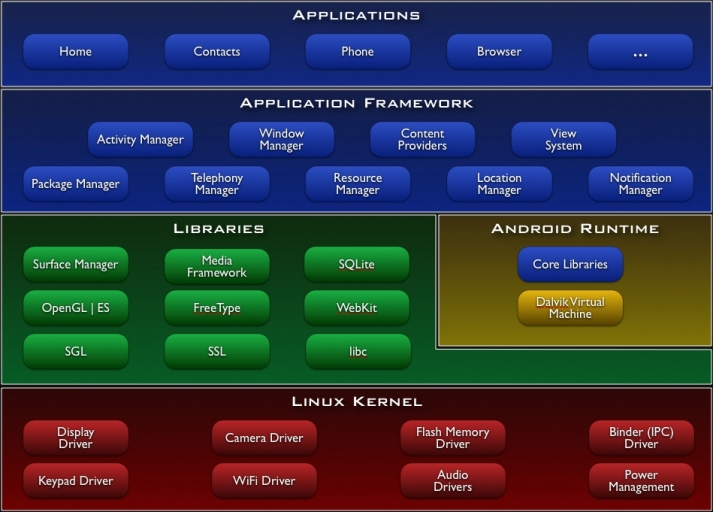
\includegraphics[height=6.5cm]{figs/android-architecture}
\end{center}
\end{frame}

\begin{frame}
\frametitle{HTC Dream - G1}

\begin{columns}
\begin{column}{0.63\textwidth}

\begin{itemize}
\item Qualcomm MSM7201A a 528 MHz
\item RAM: 128 MB RAM - ROM: 256 MB
\item Touch screen: 3,17 inches
\item Camera: 3.1 Mp
\item GPS, accelerometers and compass
\item QUERTY keyboard
\item HTC Dream - G1 (market by Movistar)
\end{itemize}
\end{column}

\begin{column}{0.4\textwidth}
\begin{center}
  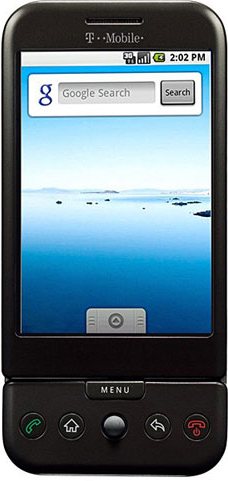
\includegraphics[height=5.5cm]{figs/tmobile-g1}
\end{center}
\end{column}
\end{columns}
\end{frame}


\begin{frame}
\frametitle{HTC Magic - G2}

\begin{columns}
\begin{column}{0.5\textwidth}

\begin{itemize}
\item Restyling HTC Dream(G1)

\item Hardware very similar to HTC Dream(G1)
\item RAM: 192 MB RAM - ROM: 512 MB
\item Trackball with Enter button (Blackberry)
\item Software: Cupcake release (currently, 2.2)
\item HTC Magic -G2 (market by Vodafone)
\end{itemize}
\end{column}

\begin{column}{0.5\textwidth}
\begin{center}
  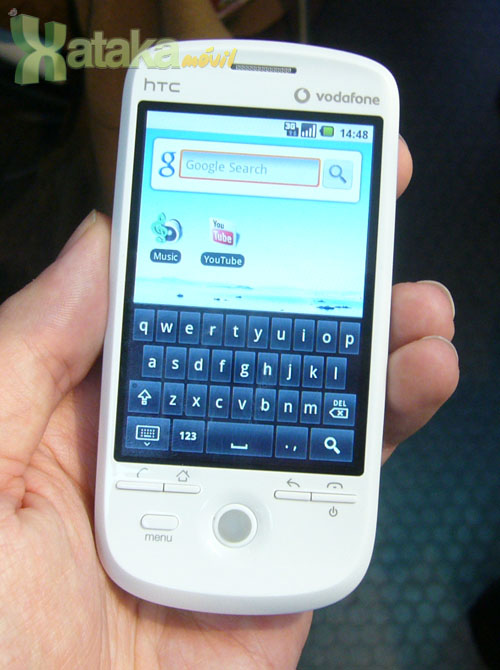
\includegraphics[height=5.5cm]{figs/htc-magic}
  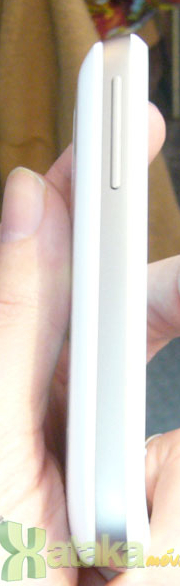
\includegraphics[height=5.5cm]{figs/htc-magic-2}
\end{center}
\end{column}
\end{columns}
\end{frame}


\begin{frame}
\frametitle{Nexus One}

\begin{columns}
\begin{column}{0.5\textwidth}

\begin{itemize}

\item The Google phone
\item QUALCOMM QSD 8250, 1Ghz
\item RAM: 512 MB - ROM: 512 MB
\item Proximity and light sensor
\item Software: Android 2.3.3
\item Second micro for noise cancellation
\item Sales online
\end{itemize}
\end{column}

\begin{column}{0.5\textwidth}
\begin{center}
  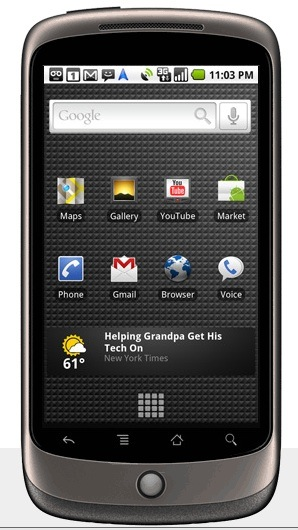
\includegraphics[height=5.5cm]{figs/nexus-one}
\end{center}
\end{column}
\end{columns}
\end{frame}

\begin{frame}
\frametitle{Samsung Galaxy S}

\begin{columns}
\begin{column}{0.5\textwidth}

\begin{itemize}

\item S5PC110 con PowerVR SGX540, 1Ghz
\item RAM: 512 MB - ROM: 650 MB
\item SuperAmoled Screen, 4''
\item Software: Android 2.3
\item Bluetooth 3.0
\item Recording video at 720p
\end{itemize}
\end{column}

\begin{column}{0.5\textwidth}
\begin{center}
  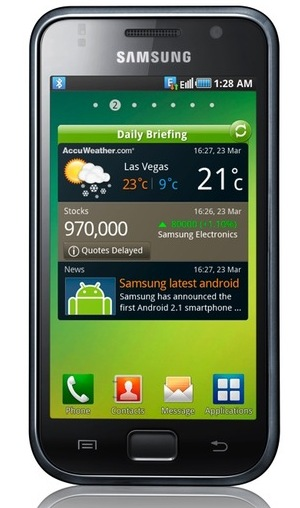
\includegraphics[height=5.5cm]{figs/samsung-galaxy-s}
\end{center}
\end{column}
\end{columns}
\end{frame}


\begin{frame}
\frametitle{Samsung Galaxy Nexus}

\begin{columns}
\begin{column}{0.5\textwidth}

\begin{itemize}

\item The most advanced Android
\item Procesador TI OMAP 4460 dual-core 1.2 GHz
\item RAM: 1GB - ROM: 16GB
\item SuperAmoled Screen, 4,65''
\item Software: Android 4.0
\item NFC, noise cancelation
\item Barometro
\end{itemize}
\end{column}

\begin{column}{0.5\textwidth}
\begin{center}
  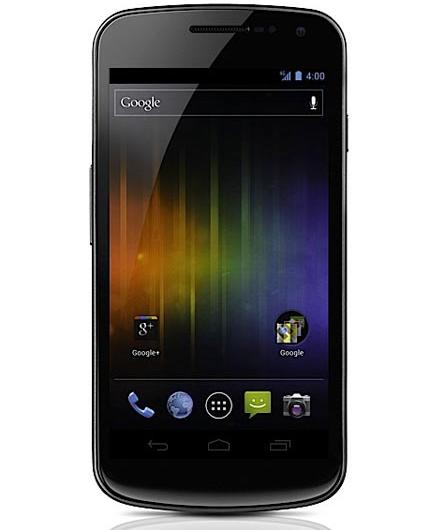
\includegraphics[height=5.5cm]{figs/samsung-galaxy-nexus1}
\end{center}
\end{column}
\end{columns}
\end{frame}



\begin {frame}
\frametitle{Android Firmware}

\begin{itemize}
\item Release 1.1: Installed in G1 and ADP (Android Developer Phone)
\item Release 1.5 (Cupcake); Installed in G2.
\item Release 1.6 (Donut)
\item Release 2.0 (Eclair) Motorola Droid - Motorla Milestone
\item Release 2.1 (Eclair) Samsung Galaxy S
\item Release 2.2 (Froyo): Nexus One
\item Release 2.3.X (Gingerbread)
\item Release: 3.0 (Honeycomb)
\item Last Release: 4.0 (IceCreamSandwich)
\end{itemize}

\begin{center}
\htmladdnormallink{Android Timeline: http://www.androidacademy.com/4-android-timeline}{http://www.androidacademy.com/4-android-timeline}
\end{center}

\end{frame}


\begin{frame}
\frametitle{Android Market}

\begin{columns}
\begin{column}{0.6\textwidth}
\begin{itemize}
\item Anyone can publish applications
\item Applications do not need to be approved by Google
\item Applications can be by free or at a cost/price (depends of country)
\item Voting system similar to youtube
\end{itemize}
\end{column}

\begin{column}{0.4\textwidth}
\begin{center}
  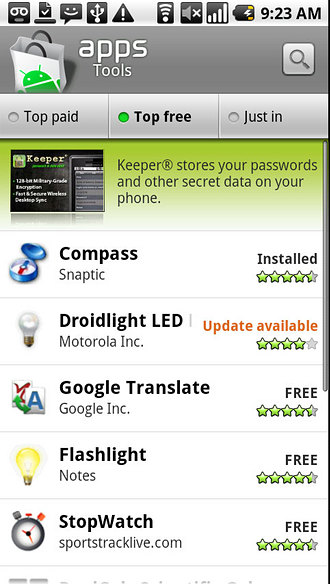
\includegraphics[height=5.5cm]{figs/android-market}
\end{center}

\end{column}
\end{columns}
\end{frame}


\section{Killer Applications}

\begin{frame}
\frametitle{Google Streets View}

\begin{columns}

\begin{column}{0.6\textwidth}
\begin{itemize}
\item Developed by Google
\item Another step in google maps
\item Integrated into Android system
\end{itemize}

\begin{center}
\htmladdnormallink{Link to video}{http://www.youtube.com/watch?v=4PRfVKzuUJ4}
\end{center}
\end{column}

\begin{column}{0.4\textwidth}
\begin{center}
  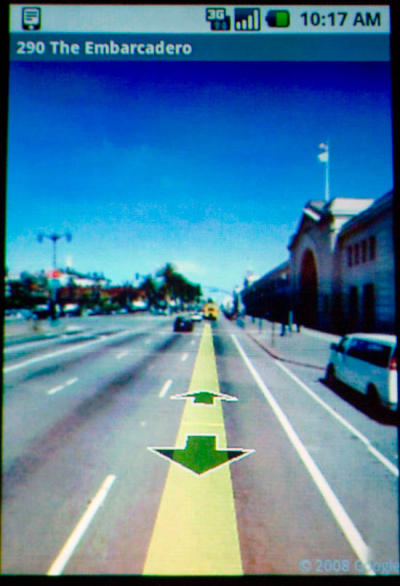
\includegraphics[height=4.5cm]{figs/googleStreetsView.jpg}
\end{center}

\end{column}
\end{columns}

\end{frame}

\begin{frame}
\frametitle{WikiTude}

\begin{itemize} 
\item The first killer application in Android.
\item It is a mobile travel guide based on location based Wikipedia
\item It is a Top-50 finalist in Google's Android Developer Challenge
\item Augmented Reality based in Geo-Location (GPS and compass)
\end{itemize}

\begin{center}
\htmladdnormallink{Link to video}{http://www.youtube.com/watch?v=tpaJBu4BEuA}
\end{center}

\end{frame}



\begin{frame}
\frametitle{LibreGeoSocialApp}

\begin{center}
  
\includegraphics[height=1.5cm]{figs/LibreGeoSocialApp}
\end{center}
\begin{itemize}
\item It is an android application that exploits all the functionality
  of mobile social network with augmented reality (AR) interface.
\item Research about gps, compass and accelerometers, AR
\item The location in the mobile has a lot of power
\item The mobile concept is changing
\end{itemize}

\begin{center}
\htmladdnormallink{See application video}{http://www.youtube.com/watch?v=GTgocMYUiK8}

\end{center}

\end{frame}


%\begin{frame}
%\frametitle{LibreGeoSocialApp: Features}
%
%\begin{itemize}
%\item Register and login users
%\item Geo-Located through GPS and WIFI signal
%\item Obtain nearby places information of channels as 11870 and
%  Panoramio
%\item Find friends by closeness and see his position
%\item Upload geo-located notes 
%\item Upload geo-located photos
%\end{itemize}
%
%\begin{center}
%\htmladdnormallink{Video}{file:///home/rocapal/libresoft/social-network/videos/LibreSocialApp_14-01-2009.mpg}
%\end{center}
%
%\end{frame}


\section{Aspects of Community}

\begin{frame}
\frametitle{Community}

\begin{itemize}
\item Peculiar open source community: An enterprise creates a
  software
\item Works with mailing list, git, forums and blogs
\item Android isn't developed only for google people
\item SDK Section: 96 different authors
\item Core Section: 81 different authors
\item Framework Section: 283 different authors

\end{itemize}
\end{frame}

\begin{frame}
\frametitle{Android and the Linux Kernel Community}
\begin{itemize}
\item Linux 2.6.33 released without Android source code
\item Google does not arrive in time to make the necessary changes
\item Google has not intend to create a fork of Linux
\item It's expected to be integrated to version 2.8
\end{itemize}

\begin{center}
\htmladdnormallink{Polemic Forum}{http://lwn.net/Articles/372419/} \\
\htmladdnormallink{Greg Kroah-Hartman, Linux Driver Project leader }{http://www.kroah.com/log/linux/android-kernel-problems.html}
\end{center}
\end{frame}

\begin{frame}
\frametitle{Cyanogen vs Google}
\begin{itemize}
\item Cyanogen is an alternative release for android phones
\item Direct cause of the fragmentation in Android
\item Android is free software, Google Apps aren't
\item Solution: Cyanogen is distributed without Google Apps
\end{itemize}

\begin{center}
\htmladdnormallink{Official Google Note}{http://android-developers.blogspot.com/2009/09/note-on-google-apps-for-android.html} \\
\end{center}
\end{frame}


\begin{frame}
\frametitle{Fragmentation}

\begin{itemize}
\item What is the problem?
\item Many devices with differents specifications and differents
  versions of Android
\item Why does happen with Android?
\item It's a problem for consumers, developers, manufacturers, ...
\item Is there a solution?
\end{itemize}

\end{frame}

\section{Interesting Facts and Numbers}

\begin{frame}
\frametitle{Iphone vs Gphone}
\begin{center}
   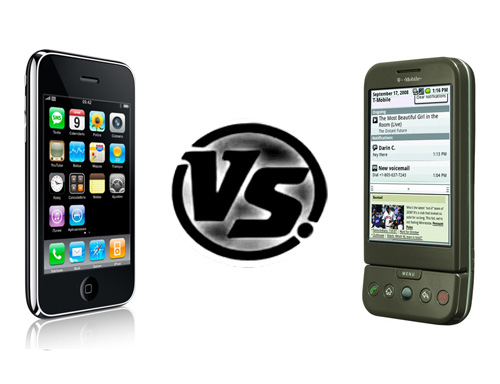
\includegraphics[height=5.5cm]{figs/iphone-vs-gphone.jpg}
\end{center}
\end{frame}


\begin{frame}
\frametitle{Iphone vs Gphone}
\begin{columns}
\begin{column}{0.45\textwidth}
* Iphone
\begin{itemize}
 \item Apple
 \item Propietary Software, Patents
 \item Best Design and Screen
 \item Memory and Battery soldier
 \item It is necessary to pay to develop and publish applications
\end{itemize}
\end{column}
\begin{column}{0.55\textwidth}
* Gphone
\begin{itemize}
 \item Google
 \item Free/Libre Software
 \item QWERTY keyboard (depending models)
 \item ADP (Android Developer Phone)
 \item Includes compass
 \item Free access to development and Market
\end{itemize}
\end{column}
\end{columns}

\end{frame}

\begin{frame}
\frametitle{Usage of Android Platforms}

\begin{center}
\hspace{0.2cm}

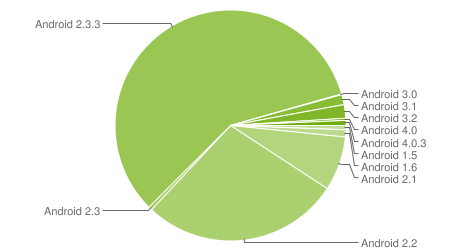
\includegraphics[height=4.0cm]{figs/android-platform}

\hspace{0.2cm}

\htmladdnormallink{News Source}{http://developer.android.com/resources/dashboard/platform-versions.html}
\end{center}
\end{frame}

\begin{frame}
\frametitle{2012: Good Year for Google}

\begin{center}
\begin{large}
 Android Devices Set To Outsell iPhones By 2012
\end{large}
\end{center}

\begin{itemize}
\item 2008: almost 162 million smartphones were sold (13.5\%)
\item 2012: Android smartphone sales will outstrip iPhone sales
\item 2013: predicts that 300 million smartphones will be sold
\item Proliferation of online stores selling specialized applications
\item \htmladdnormallink{Notice Link (Washington Post)}{http://www.washingtonpost.com/wp-dyn/content/article/2009/03/09/AR2009030902280.html}
\end{itemize} 

\end{frame}




\begin{frame}
 \frametitle{2009}

\begin{center}

\hspace{0.2cm}
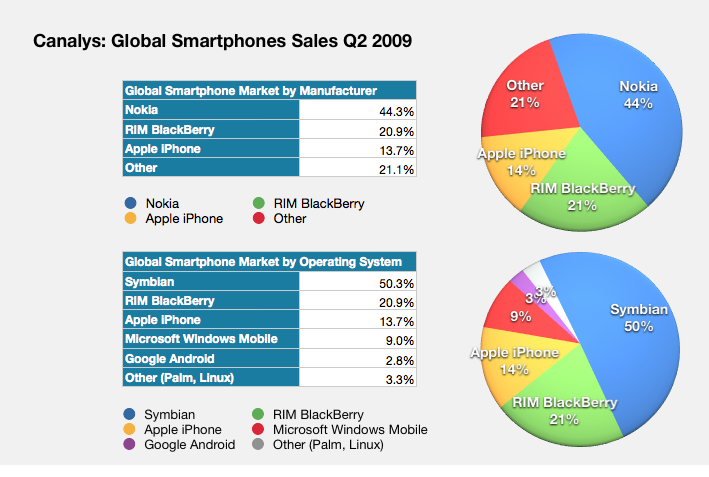
\includegraphics[height=5.0cm]{figs/global_smartphone_sales}
\hspace{0.2cm}
\end{center}

\end{frame}


%==

\begin{frame}
 \frametitle{March 2009}

\begin{center}
\begin{large}
Mobile Web Usage
\end{large}

\hspace{0.2cm}
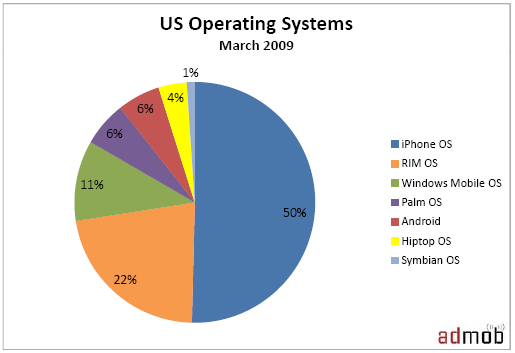
\includegraphics[height=5.0cm]{figs/mobile_web_usage0}
\hspace{0.2cm}
\end{center}

\end{frame}

%==

%\begin{frame}
%\frametitle{November 2009}

%\begin{center}
%\begin{large}
% Mobile Web Usage
%\end{large}%

%\hspace{0.2cm}

%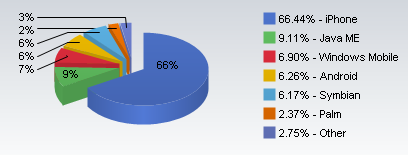
\includegraphics[height=4.0cm]{figs/mobile_web_usage}

%\hspace{0.2cm}

%\htmladdnormallink{Notice Link (PC-World)}
%                  {http://www.pcworld.com/businesscenter/article/160646/mobilephone_competition_heats_up_as_sales_slow.html}

%\end{center}

%\end{frame}

\begin{frame}
\frametitle{November 2009}

\begin{center}
\begin{large}
 Mobile Web Usage
\end{large}

\hspace{0.2cm}

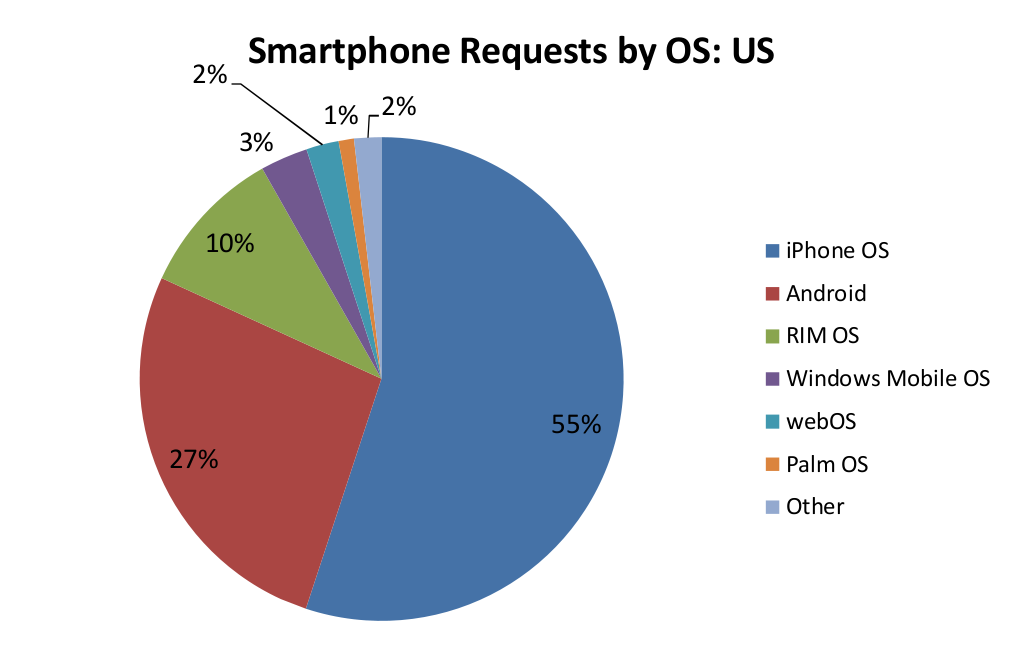
\includegraphics[height=5.0cm]{figs/admob-android-2009}


\htmladdnormallink{AdMob November 2009 Report}
                  {http://metrics.admob.com/wp-content/uploads/2009/12/AdMob-Mobile-Metrics-Nov-09.pdf}

\end{center}

\end{frame}

\begin{frame}
\frametitle{Android Outselling iPhone in Q2 2010}

\begin{center}
\hspace{0.2cm}

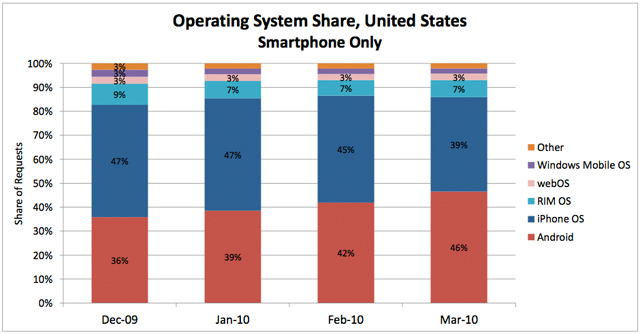
\includegraphics[height=5.0cm]{figs/iphoneosvsandroid-marzo}

\hspace{0.2cm}
\htmladdnormallink{News Link (Mashable)}{http://mashable.com/2010/05/10/android-outselling-iphone/}
\end{center}

\end{frame}


\begin{frame}
 \frametitle{October 2010}

\begin{center}
\begin{large}
Smartphone Market
\end{large}

\hspace{0.2cm}
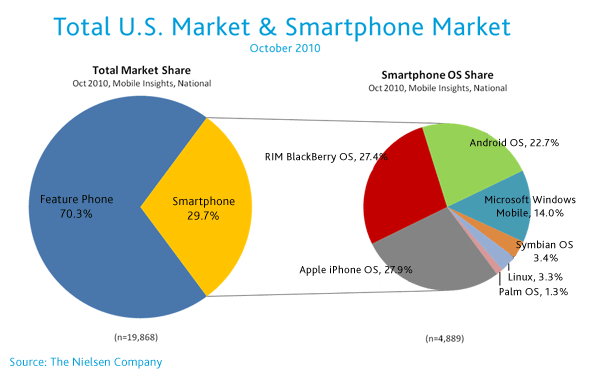
\includegraphics[height=5.0cm]{figs/mobile_web_usage2}
\hspace{0.2cm}
\end{center}

\end{frame}

\begin{frame}
 \frametitle{November 2010}

\begin{center}
\begin{large}
Mobile Web Usage
\end{large}

\hspace{0.2cm}
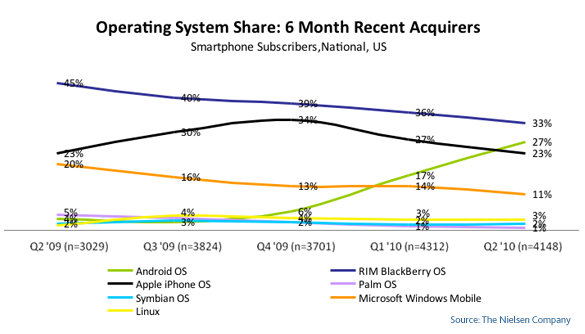
\includegraphics[height=5.0cm]{figs/mobile_web_usage3}
\hspace{0.2cm}
\end{center}

\end{frame}


\begin{frame}
 \frametitle{Q3 2011}

\begin{center}
\begin{large}
Smartphone penetration
\end{large}

\hspace{0.2cm}
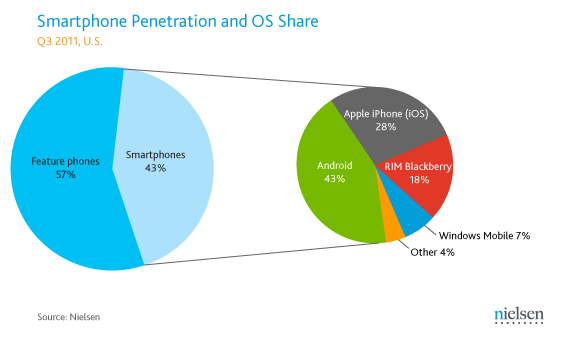
\includegraphics[height=5.0cm]{figs/mobile_web_usage4}
\hspace{0.2cm}
\end{center}

\end{frame}

\begin{frame}
 \frametitle{More curious facts}

\begin{itemize}
\item May 2010: 100.000 android devices are activated per day
\item Dic 2010: 300.000 android devices are activated per day
\item July 2011: 550.000 android devices are activated per day
\item Dec 2011: 700.000 android devices are activated per day
\end{itemize}

\begin{center}
\hspace{0.2cm}
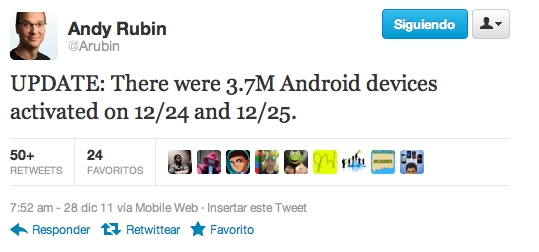
\includegraphics[height=3.0cm]{figs/andyrubin}
\hspace{0.2cm}
\end{center}


\end{frame}

%===

\begin{frame}
\frametitle{Much more than an OS for mobile}

\begin{center}
\begin{large}
Much more than an operating system for mobile
\end{large}
\end{center}
\hspace{0.2cm}

\begin{itemize}

\item Android into Archos Tablet
  \htmladdnormallink{(link)}{http://www.engadget.com/2009/02/09/archos-to-release-android-phone-tablet/} 
\item Android into Asus Eee PC \htmladdnormallink{(link)}{http://www.itwire.com/content/view/23389/1103/}
\end{itemize}

\begin{center}
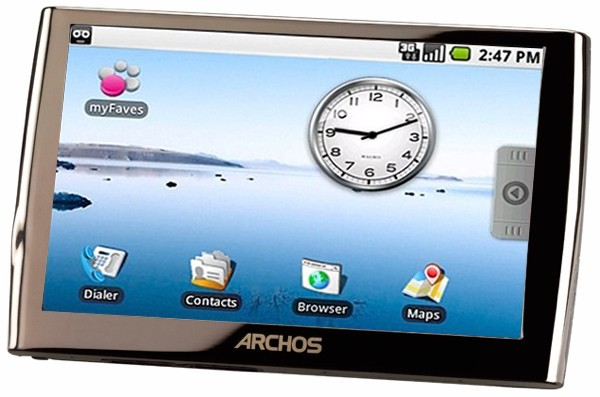
\includegraphics[height=3.0cm]{figs/archos-android}
\vspace{2.0cm}
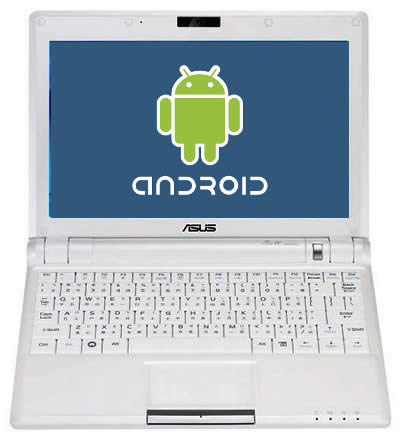
\includegraphics[height=3.5cm]{figs/eee_pc_android}
\end{center}

\end{frame}

\begin{frame}
\frametitle{Samsung Galaxy Tab}

\begin{columns}
\begin{column}{0.5\textwidth}

\begin{itemize}

\item LCD Multitouch Screen 7''
\item 1GHz Cortex A8 - PowerVR SGX540
\item 512 RAM, 16Gb with MicroSD
\item Front/Back camera
\item VideoPlayer Full HD
\item Wifi, Bluetooth 3.0, GSM!
\item \htmladdnormallink{See Video (link)}{http://www.youtube.com/watch?v=v1PO3_iqbQ8}
\end{itemize}
\end{column}

\begin{column}{0.5\textwidth}
\begin{center}
  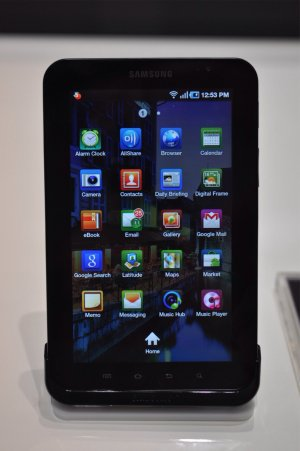
\includegraphics[height=5.5cm]{figs/galaxy-tab}
\end{center}
\end{column}
\end{columns}

\end{frame}

\section{Motivation}
\begin{frame}
\frametitle{Last News}
\begin{itemize}

\item \htmladdnormallink{Google is hiring 2.000 people in
    Europe}{http://dondodge.typepad.com/the_next_big_thing/2010/11/google-is-hiring-2000-people-how-to-get-a-job-at-google.html}

\end{itemize}

\begin{center}
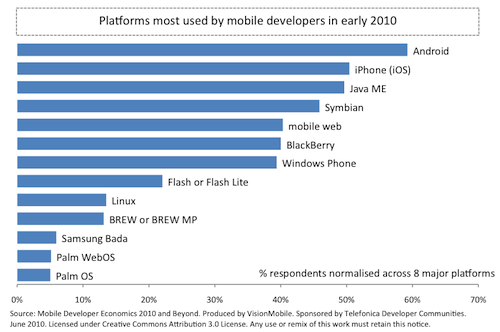
\includegraphics[height=5.0cm]{figs/DeveloperMindshare}
\end{center}
\end{frame}

\begin{frame}
\frametitle{Last News}
\begin{center}
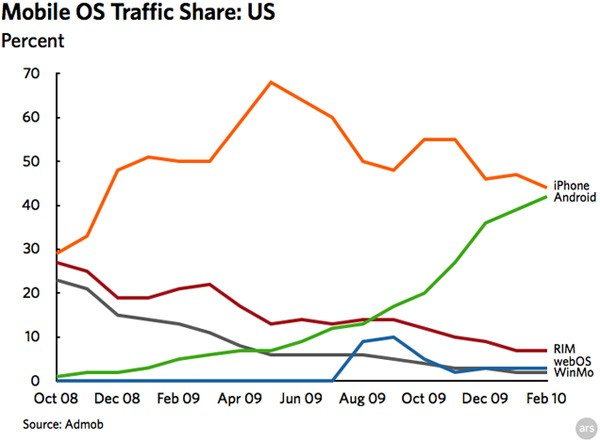
\includegraphics[height=6.0cm]{figs/MovileOSTrafficShare}
\end{center}

\end{frame}


\end{document}
